\section{Evaluating Performance}
\label{sec:results}

In this section, we test the \emph{Prediction Algorithm} presented in Section~\ref{subsec:prediction_algorithm} with the data present on the graph.

\subsection{Data Partitioning}

\subsubsection{Train Test Split}
\label{subsec:train_test_split}

As with many other classification problems, the \emph{Bayesian Algorithm} is prone to overfitting~\cite{mitchellml1997}. In this particular case, since the information presented in Section~\ref{subsec:income_homophily} shows that users tend to communicated with users of the same socioeconomic level, by running the algorithm in the complete data and using the same users as part of the features and of the labels, we would erroneously be having more data per user than we would have when modelling the problem.

An easy way to avoid this problem is by doing a simple \emph{Train Test Split}, where the data in $B$ is separated into two disjoint groups, $B = B_{\train} \cup B_{\test}$ and $B_{\train} \cap B_{\test} = \varnothing$, where $\left| B_{\train} \right| = \sfrac{4}{5} \cdot \left| B \right|$ and $\left| B_{\test} \right| = \sfrac{1}{5} \cdot \left| B \right|$.

\subsubsection{Erasing Uninformative Data}

Given that $\left| B \right| \ll \left| V \right|$ and that $G$ is sparse, the vast majority of users don't have any kind of contact with users of the bank. For this reason it's useless to evaluate the performance of the algorithm using all the nodes, and therefore the \emph{Testing Set} used in this thesis will instead focus on the bank users that have at least one contact with another bank user. This approach is formalized in Equation~\ref{eq:inner_graph}.

\begin{equation}
\label{eq:inner_graph}
\begin{gathered}
\hat{E} = \left\{ e \in E \mid e_o \in B_{\train} \lor e_d \in B_{\train} \right\} \\
\hat{B}_{\test} = B_{\test} \cap \left( \hat{E}_o \cup \hat{E}_d \right)
\end{gathered}
\end{equation}

This approach works perfectly when $\varpi = \contacts$. However, it's possible that for other values of $\varpi$ there won't be any information available in $\hat{B}_{\test}$ in the case of users who either didn't receive any call from a bank user or didn't receive any message.

The equations~\ref{eq:inner_graph_call} and~\ref{eq:inner_graph_sms} formalize new variables to use for informative data in those cases.

\begin{equation}
\label{eq:inner_graph_call}
\begin{gathered}
\hat{E}^{\calls} = \left\{ e \in E \mid e_c > 0 \land \left( e_o \in B_{\train} \lor e_d \in B_{\train} \right) \right\} \\
\hat{B}^{\calls}_{\test} = B_{\test} \cap \left( \hat{E}^{\calls}_o \cup \hat{E}^{\calls}_d \right) \\
\end{gathered}
\end{equation}

\begin{equation}
\label{eq:inner_graph_sms}
\begin{gathered}
\hat{E}^{\sms} = \left\{ e \in E \mid e_s > 0 \land \left( e_o \in B_{\train} \lor e_d \in B_{\train} \right) \right\} \\
\hat{B}^{\sms}_{\test} = B_{\test} \cap \left( \hat{E}^{\sms}_o \cup \hat{E}^{\sms}_d \right)
\end{gathered}
\end{equation}

\subsubsection{Rebalancing Labels}
\label{subsec:rebalancing_labels}

Since the testing data $B_{\test}$ was a random subsample of a balanced set (see Section~\ref{subsec:train_test_split} and Section~\ref{subsec:discrimination_by_wealth}), it was also balanced itself\maybe{Make sure $B$ refers only to bank users \textbf{in the telco}}. However, since \emph{High Income} users tend to communicate more often than \emph{Low Income} ones, $\hat{B}_{\test}$ is unbalanced and has a significant bias for high-income users.

Since the income categories tend to be balanced in the real world, this isn't wanted. However, since it's not necessary to use the entire \emph{Testing Set} for testing the algorithm, a simple way would be to create a new, balanced, and final testing set, $\Upsilon \subseteq \hat{B}_{\test}$ containing all users from $\hat{B}_{\test}$ \emph{Low Income}, along with a random sample of the same size with \emph{High Income}.

\begin{equation}
\label{eq:upsilon}
\begin{gathered}
\begin{aligned}
\Upsilon^{\low} &= \hat{B}_{\test} \cap H_1 \\
\Upsilon^{\high} &\subseteq \hat{B}_{\test} \cap H_2
\end{aligned} \\
\left| \Upsilon^{\low} \right| = \left| \Upsilon^{\high} \right| \\
\Upsilon = \Upsilon^{\low} \cup \Upsilon^{\high}
\end{gathered}
\end{equation}

$\Upsilon$ will be the only \emph{Testing Set} used from now on, while $B_{\train}$ will be used as training set.

Additionally, the sets $\Upsilon^{\calls}$ and $\Upsilon^{\sms}$ refer to similar sets which are taken from users from the \emph{Testing Set} that had at least one call or sent at least one SMS, respectively, to another user in the \emph{Training Set}.

\subsubsection{Set Magnitudes}

While the new set $\Upsilon$ contains significantly less users than the original set $B$, it still has a sufficient amount of people to make a prediction. Table~\ref{tab:partition_numbers} shows the number of users that remain after every trim used in this Subsection, along with the ratio of users which we would be able to assign an \emph{Income Category} using these datasets assuming the real data is equally distributed from the \emph{Test Data}.

\begin{table}
\centering
\begin{tabular}{l r r r c}
\toprule
Set & Total Size & High Income & Low Income & Ratio \\
\midrule
$B$ & \num{5402959} & \num{2702628} & \num{2700331} & \NA{} \\
$B_{\test}$ & \num{1080592} & \num{540526} & \num{540066} & \NA{} \\
$\hat{B}_{\test}$ & \num{53691} & \num{35215} & \num{18476} & \num{1.000} \\
$\Upsilon$ & \num{36952} & \num{18476} & \num{18476} & 1.000 \\
$\Upsilon^{\calls}$ & \num{30715} & \num{15653} & \num{15062} & 0.831 \\
$\Upsilon^{\sms}$ & \num{11909} & \num{6046} & \num{5863} & 0.322 \\
\bottomrule
\end{tabular}
\caption{Amount of users in the \emph{Testing Set} after trimming it several times to prevent overfitting while keeping the labels balanced}
\label{tab:partition_numbers}
\end{table}

\newpage

\subsection{Choosing the best $\Theta$}

Choosing a good value of $\Theta$ is an essential step in creating a correct algorithm since it's the most important constant of Equation~\ref{eq:beta_theta_ppf}, one of the crucial parts for finding the category of an user.

As explained in Section~\ref{subsec:modelling_users}, it's convenient to use \emph{Jeffrey's Prior} as the prior distribution for this variable. However, knowing how it will affect the prediction of the category of each $v$ for every $\varpi$ will allow us to get a good posterior value.

The main hypotheses tested in this part of the theses were two assumptions.

\begin{enumerate}
	\item The optimal value of $\Theta$ will be the same for any $\varpi$.
	\item Overlooking extreme values, the value of $\Theta$ won't improve or deteriorate the prediction.
\end{enumerate}

As Table~\ref{tab:besttheta} and Figure~\ref{fig:theta} show, both hypotheses are false.

\begin{figure}
\centering
\includegraphicsmaybe{figures/theta.png}
\caption{The \emph{Area Under the Curve} for different $\Theta$ and every possible $\varpi$. This is the preliminary version of the analysis seen in Section~\ref{subsec:algorithm_performance}}.
\label{fig:theta}
\end{figure}

\setlength{\tabcolsep}{3pt}
\begin{table}
\centering
\begin{tabular}{>{\bfseries}l r r}
	\toprule
	$\varpi$ & Opt. $\Theta$ & AUC \\
	\midrule
	contacts & \num{0.394} & \num{0.746} \\
	calls & \num{0.428} & \num{0.724} \\
	time & \num{0.001} & \num{0.718} \\
	sms & \num{0.428} & \num{0.715} \\
	\bottomrule
\end{tabular}
\caption{Optimal $\Theta$ for each $\varpi$}
\label{tab:besttheta}
\end{table}

The \emph{Area Under the Curve} is a good way to analyze the performance of the algorithm with given hyperparameters since it provides a good equillibrium between \emph{Precision} and \emph{Recall}, and it's not necessary to establish a $\tau$ to get these values.

In this analysis we can see that there are different optimal $\Theta$ for every $\varpi$, contradicting the first hypothesis althrough the best value seems to be the same for $\varpi = \calls$ and $\varpi = \sms$. The reason for this equality remains a mystery.

Additionally, there is a significant difference between the values of $\Theta$ on all input types, contradicting the second one, except for $\varpi = \etime$. This is probably caused because the calling time is a lot more varied than with the other statistics, as is shown in Section~\ref{subsec:time_infer}.

\subsection{Algorithm Performance on All Users}
\label{subsec:algorithm_performance}

The \emph{Bayesian Algorithm} will be ran for every $\varpi \in \left\{ \contacts, \calls, \etime, \sms \right\}$. For every possible configuration, we present 3 plots for the optimal $\Theta$.

\begin{itemize}
	\item A \textbf{histogram} presenting the distribution of the $p_v$ values which result from applying Equation~\ref{eq:beta_theta_ppf} presented in Section~\ref{subsec:modelling_users} to each distinct \emph{Beta Distribution}.
	\item An \textbf{Receiver Operating Characteristic Curve}, showing the tradeoff of \emph{False Positive Rate} to \emph{True Positive Rate} when selecting every possible $\tau$. The \emph{Area Under the Curve} is marked, as this is the metric that is being maximized when selecting the correct $\varpi$.
	\item An \textbf{Accuracy Curve}, which shows the \emph{Accuracy} of the predictor by its \emph{False Positive Rate}. $\tau$ is chosen as to maximize this value.
\end{itemize}

\subsubsection{Inferring by Calls}
\label{subsec:calls_infer}

\begin{center}
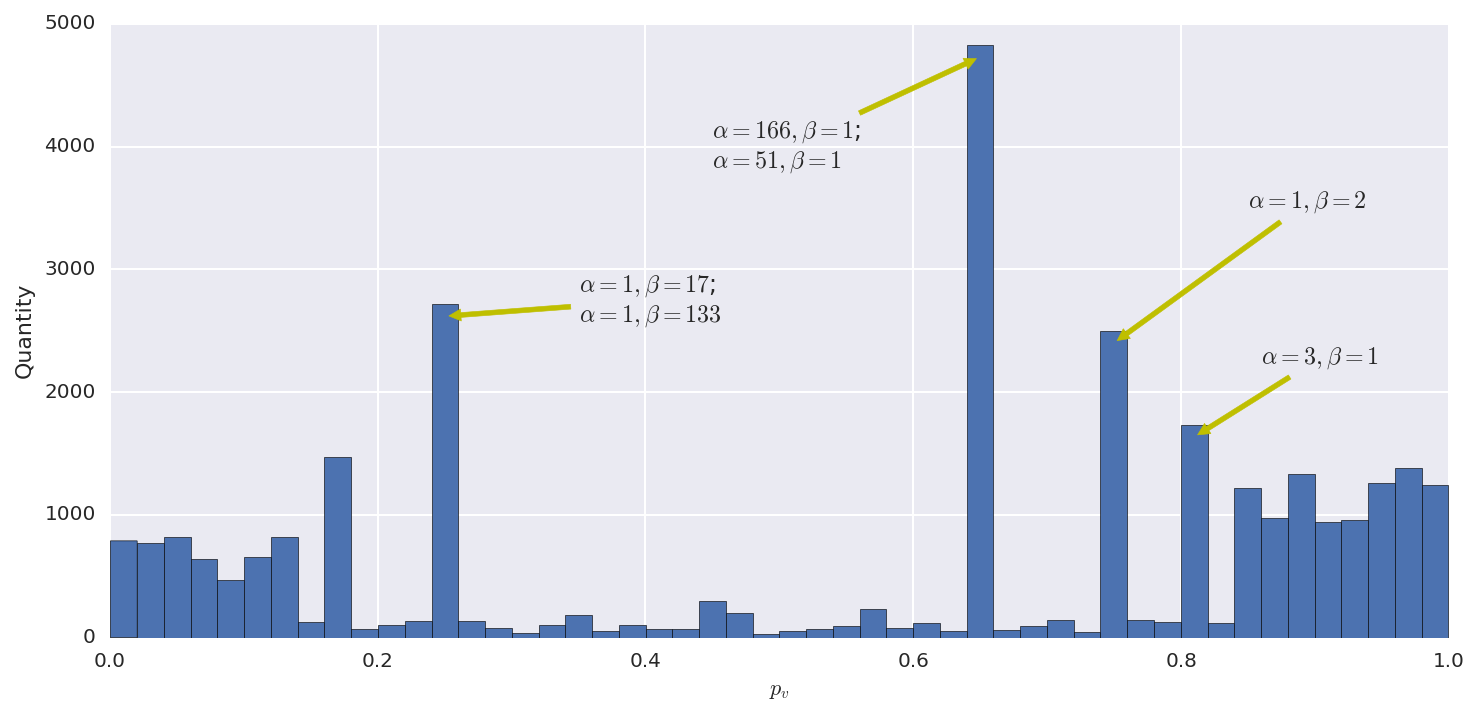
\includegraphics[width=\textwidth]{figures/bayes/hist_calls.png}
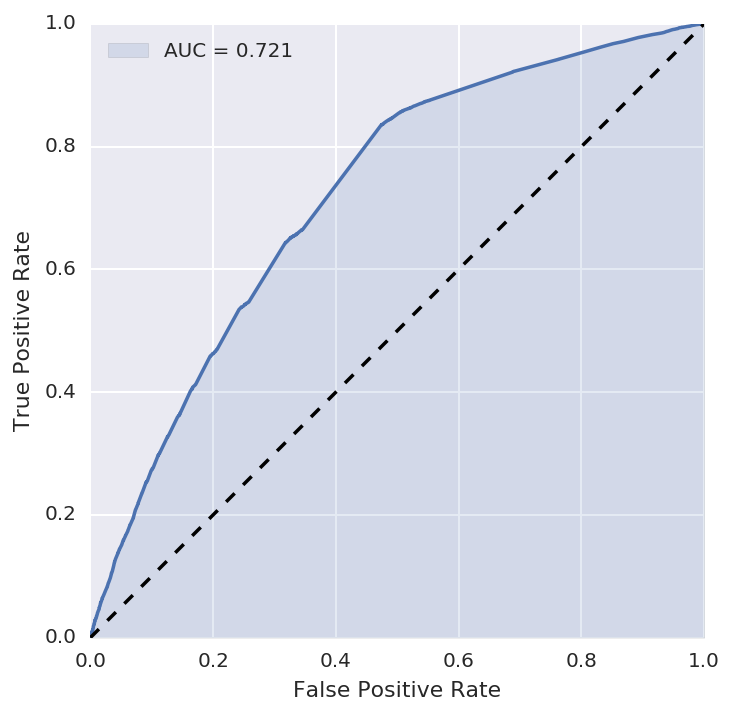
\includegraphics[width=.49\textwidth]{figures/bayes/roc_calls.png}
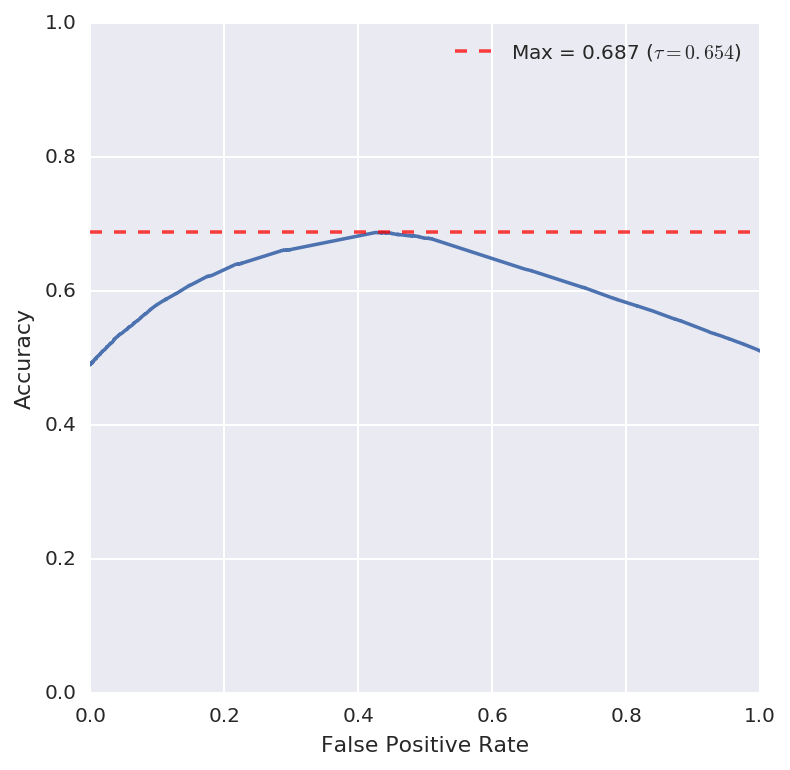
\includegraphics[width=.49\textwidth]{figures/bayes/accuracy_calls.png}
\end{center}

When $\varpi = \calls$ and the data is analyzed using $\Upsilon^{\calls}$ as \emph{Testing Set}, the \emph{Inverse Cumulative Distribution Function} has several peaks containing groups of users with similar amount of calls, and the data has a significant bias towards calls towards calls to \emph{Low Income} users.

After analyszing the data, we find that the \emph{Area Under the Curve} using this method is of \num{0.724}, which is significantly higher than all the naïve and \emph{Machine Learning} methods presented in the later Section~\ref{sec:comparison}.

To maximize accuracy, setting $\tau = 0.654$ results in a predictor where $\Accuracy = 0.687$. Additionally, that value of $\tau$ results in $\Precision = 0.653$, $\Recall = 0.815$, $F_1 = 0.725$, and $F_4 = 0.804$.

\subsubsection{Inferring by Time}
\label{subsec:time_infer}

\begin{center}
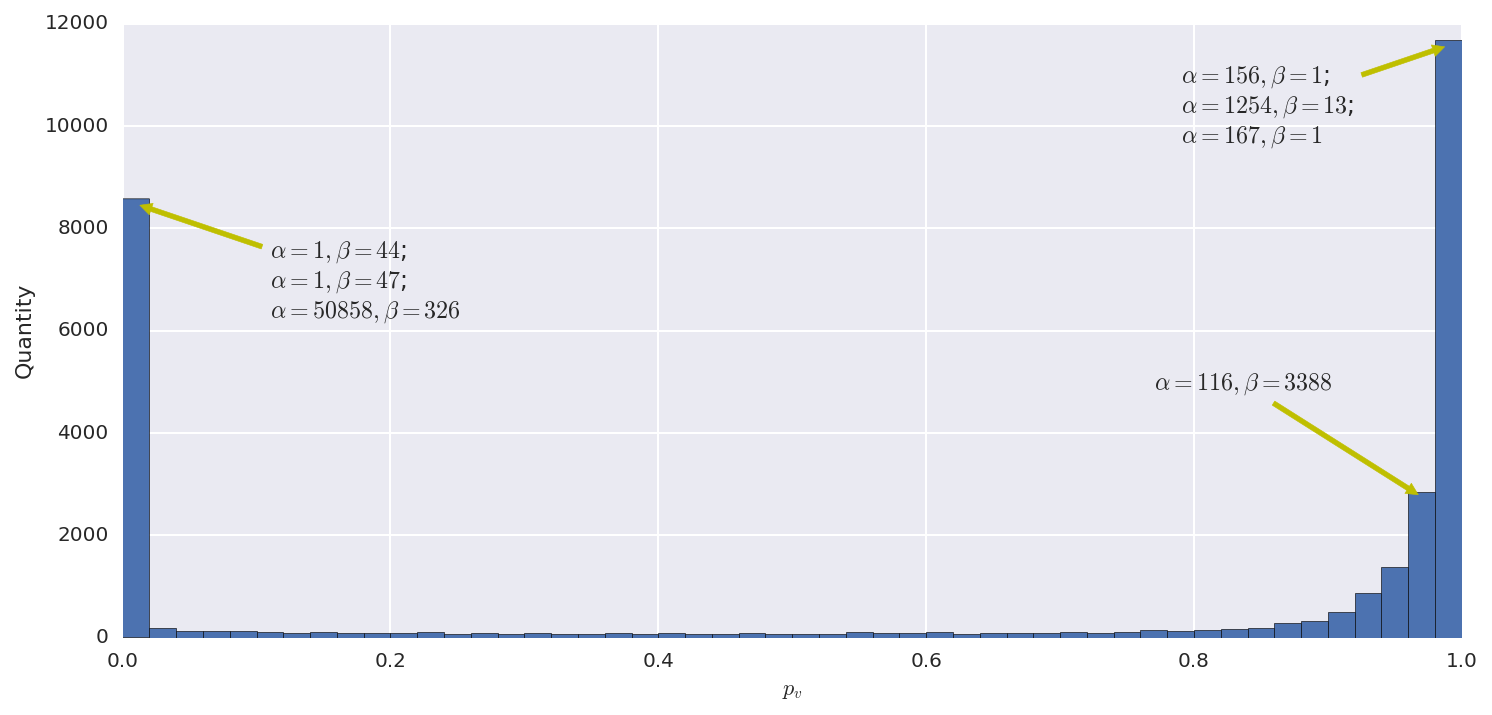
\includegraphics[width=\textwidth]{figures/bayes/hist_time.png}
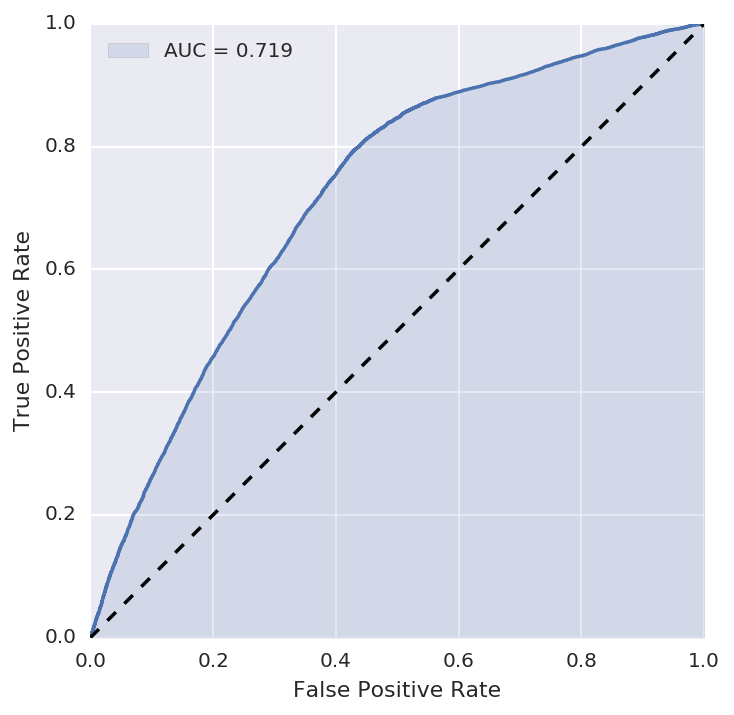
\includegraphics[width=.49\textwidth]{figures/bayes/roc_time.png}
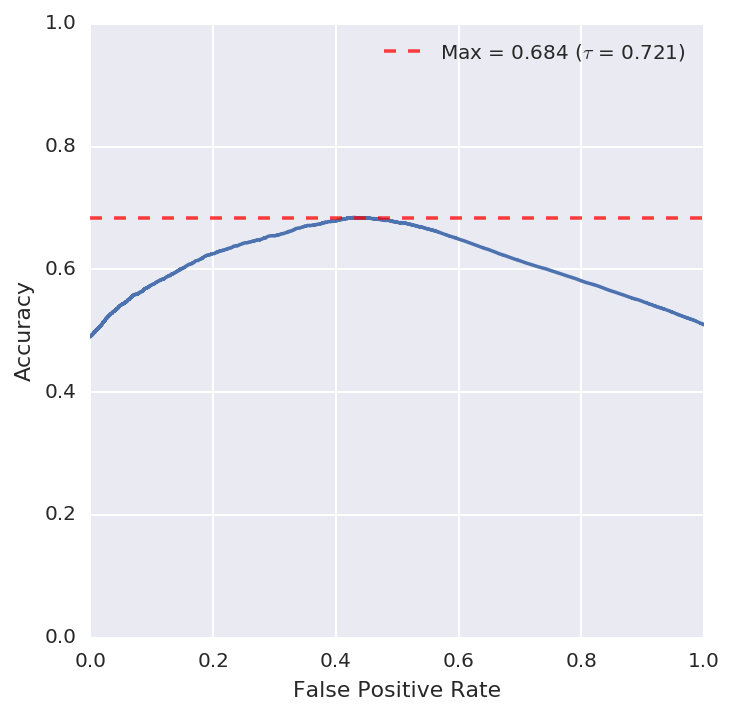
\includegraphics[width=.49\textwidth]{figures/bayes/accuracy_time.png}
\end{center}

When $\varpi = \etime$ and the data is analyzed using $\Upsilon^{\calls}$ as \emph{Testing Set}, there are two big clusters of data at the edges. The reason for these is that, as shown by Figure~\ref{fig:timeheatmap}, the majority of users only call either \emph{High Income} or \emph{Low Income} users. For completeness sake, this test is run again in Section~\ref{fig:time_infer_positive} only for the subset $\hat{\Upsilon}^{\calls} \subseteq \Upsilon^{\calls}$ which have at least one call to users of each income category; however, while this makes the histogram more equitative taking out the users with SMS to both categories (whose users tend to be in that same category) makes all the metrics lower.

The \emph{Area Under the Curve} of this inference mechanism is $\AUC = 0.718$, which is lower than the one for the calls in Section~\ref{subsec:calls_infer}. The \emph{Accuracy Curve} is unsurprisingly similar to that one, and even the \emph{Accuracy} at $\tau = 0.722$ is the same. This is probably a result of using the same dataset as that section, and the fact that there is an obvious correlation between total talking time and total calls, shown in Figure~\ref{fig:call_time}.

That value of $\tau$ also results in a predictor where $\Accuracy = 0.684$, $\Precision = 0.649$, $\Recall = 0.819$, $F_1 = 724$, and $F_4 = 807$.

\subsubsection{Inferring by SMS}
\label{subsec:sms_infer}

\begin{center}
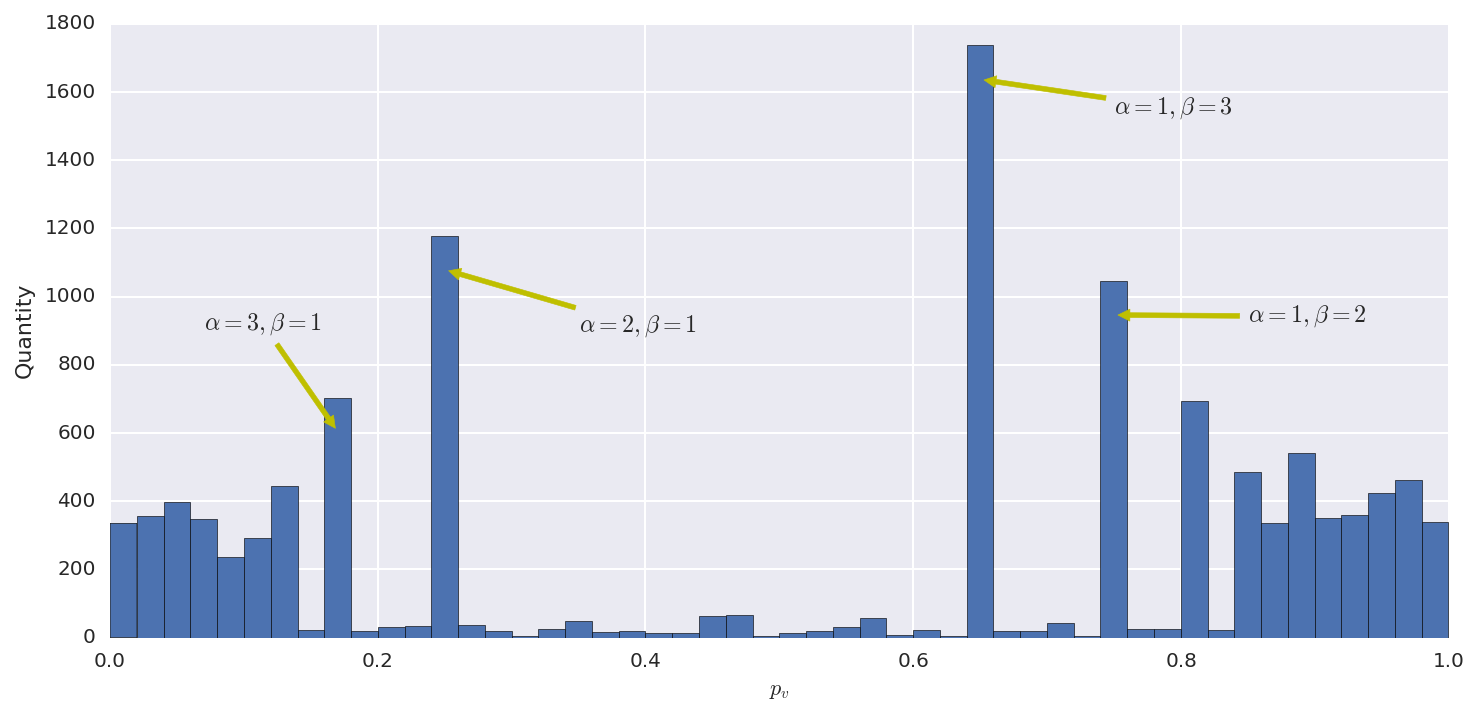
\includegraphics[width=\textwidth]{figures/bayes/hist_sms.png}
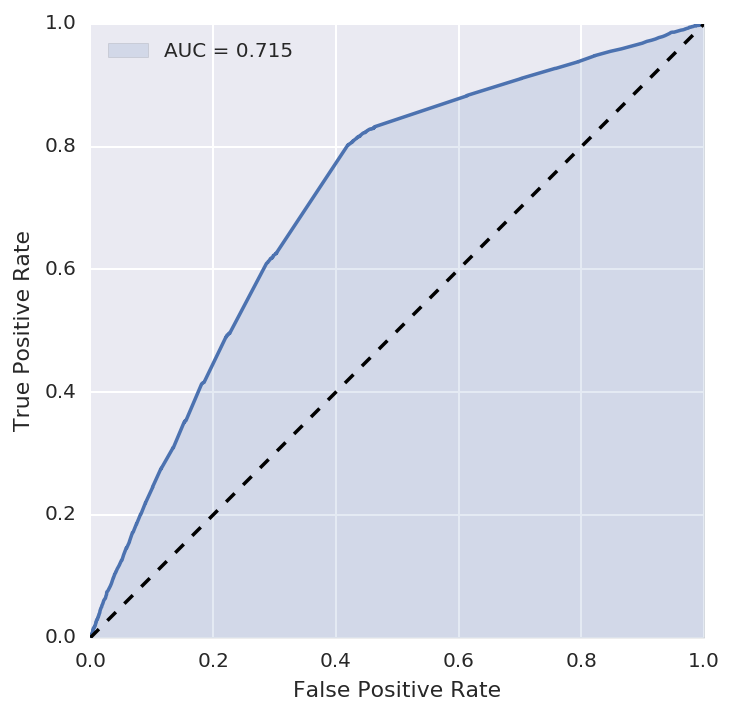
\includegraphics[width=.49\textwidth]{figures/bayes/roc_sms.png}
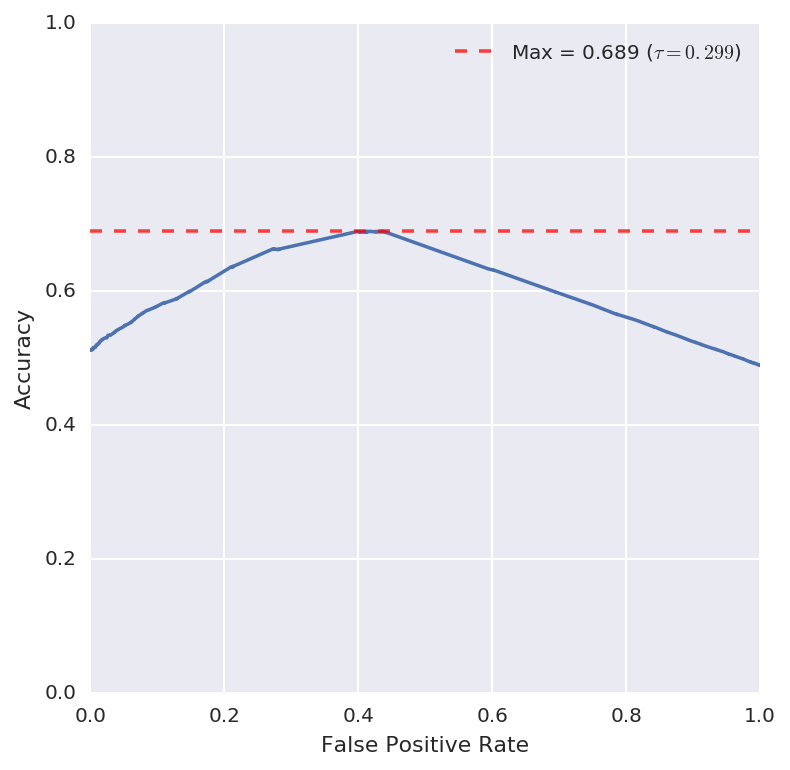
\includegraphics[width=.49\textwidth]{figures/bayes/accuracy_sms.png}
\end{center}

Since the total amount of SMS is much lower than the amount of calls, the peaks of the result of the \emph{Inverse Cumulative Functions} of the \emph{Beta Distribution} applied on $\Upsilon^{\sms}$ that happen with the majority of users that have few of both are located closer to the center than in Section~\ref{subsec:call_infer} and Section~\ref{subsec:time_infer}. This makes some interesting cases if $\varpi = \sms$ is chosen, since the distribution is different than in the other cases.

In particular, this gives an $\AUC = 0.715$, which is lower than both in the case of \emph{Calls} and \emph{Time}. Interesingly, the maximum \emph{Accuracy} at $\tau = 0.299$ is slightly higher than both of the other cases; this is probably a side-effect of the fact that $\left| \Upsilon^{\sms} \right| < \left| \Upsilon^{\calls} \right|$.

Additionally, $\Precision = 0.696$, $\Recall = 0.186$, $F_1 = 0.293$, and $F_4 = 0.194$.

\subsubsection{Inferring by Contacts}
\label{subsec:contacts_infer}

\begin{center}
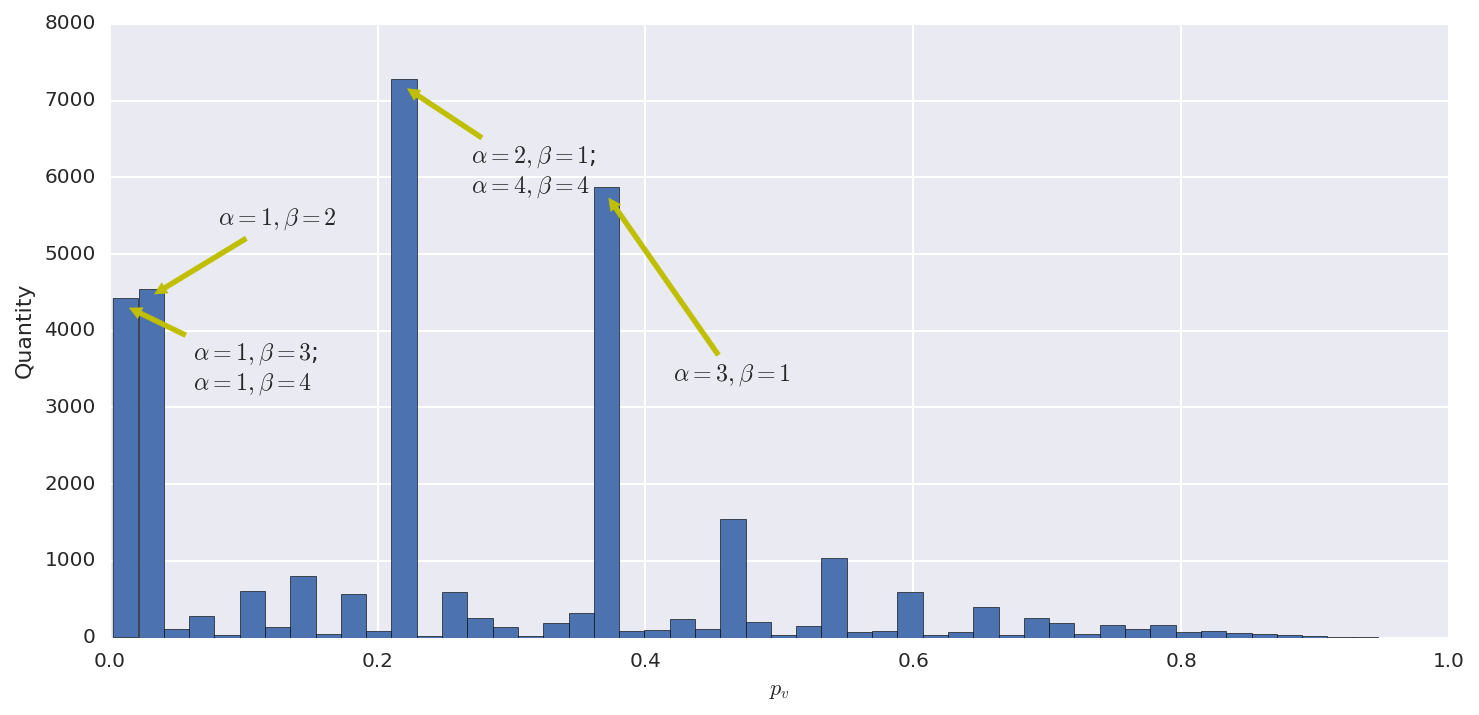
\includegraphics[width=\textwidth]{figures/bayes/hist_contacts.png}
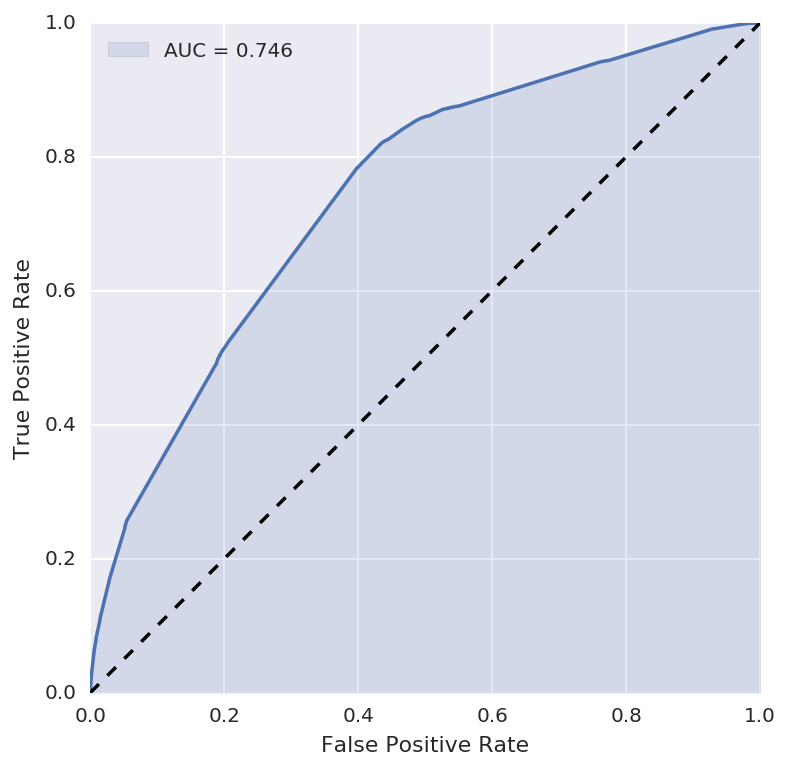
\includegraphics[width=.49\textwidth]{figures/bayes/roc_contacts.png}
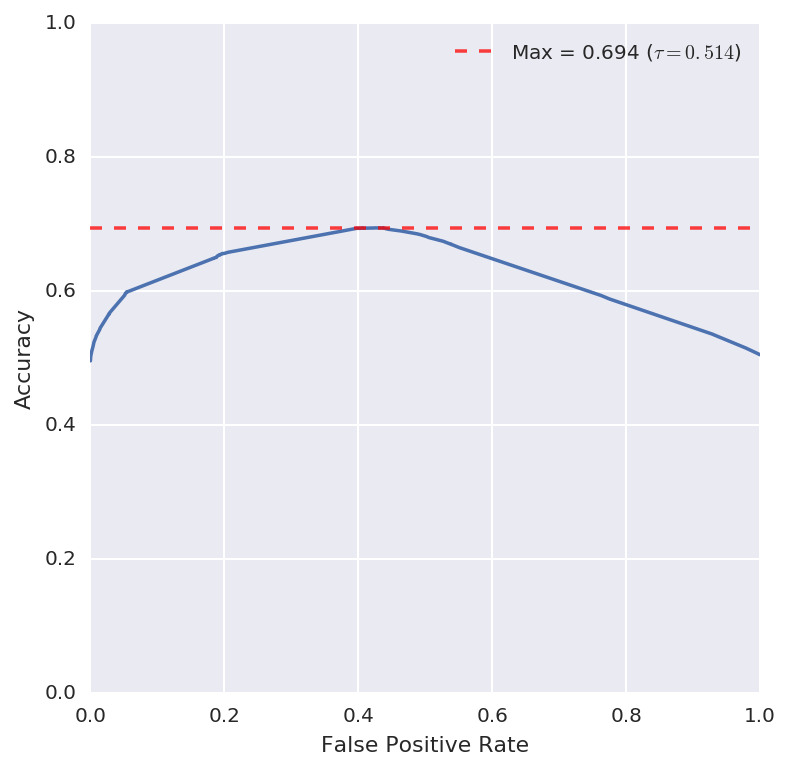
\includegraphics[width=.49\textwidth]{figures/bayes/accuracy_contacts.png}
\end{center}

When $\varpi = \contacts$ it's possible to get a pattern similar to the one shown in Section~\ref{subsec:sms_infer} when $\varpi = \sms$, where the majority of users have relatively few contacts and the peaks in the histogram. Additionally, since the total amount of contacts is logarithmically distributed (as shown in Figure~\ref{fig:contact_distribution}), and people with \emph{High Income} tend to have more contacts in general, there peaks are clustered in areas with low $p_v$ (where the majority of calls are made to \emph{Low Income} users), near the middle (where the calls are mostly equally distributed), but not at high $p_v$; this last section would belong to the few users with many calls to \emph{High Income} users.

Using this method it's possible to find that $\AUC = 0.746$, which is higher than all the other methods presented in Section~\ref{subsec:algorithm_performance}. Additionally, when selecting $\tau = 0.514$, $\Accuracy = 0.694$ which is higher than the maximum \emph{Accuracy} in all other methods. These metrics, combined with the fact that $\Upsilon$ contains every user in the \emph{Testing Set}, result in the fact that $\varpi = \contacts$ is uambiguously the best way to classify the data for the algorithm. Additionally, $\Precision = 0.556$, $\Recall = 0.792$, $F_1 = 0.723$, and $F_4 = 0.783$.

\subsubsection{Final Results}

Table~\ref{tab:bayesresults} presents every metric discussed in Section~\ref{subsec:mlmetrics} for the optimal $\Theta$ and $\tau$ for every $\varpi$.

\begin{table}
\centering
\begin{tabular}{>{\bfseries}l >{\hspace{1em}}r r >{\hspace{1em}}r r r r r r}
\toprule
$\varpi$ & \ct{Opt. $\Theta$} & \ct{Opt. $\tau$} & \ct{Acc.} & \ct{Prec.} & \ct{Rec.} & \ct{AUC} & \ct{F\textsubscript{1}} & \ct{F\textsubscript{4}} \\
\midrule
calls    & 0.428 & 0.654 & 0.686 & 0.654 & 0.816 & 0.724 & 0.726 & 0.804 \\
time     & 0.001 & 0.722 & 0.681 & 0.652 & 0.806 & 0.718 & 0.721 & 0.795 \\
sms      & 0.428 & 0.299 & 0.688 & 0.648 & 0.789 & 0.715 & 0.712 & 0.779 \\
contacts & 0.394 & 0.514 & 0.693 & 0.665 & 0.792 & 0.746 & 0.723 & 0.783 \\
\bottomrule
\end{tabular}
\caption{Metrics for the Bayesian algorithm using every user in $\Upsilon$}
\label{tab:bayesresults}
\end{table}

In particular, the results show that using \emph{Contacts} as the predictor for the \emph{Bayesian Algorithm} results in a signicantly higher \emph{Area Under the Curve} and a higher \emph{Accuracy}.

\subsection{Algorithm Performance of Users with at least 3 Contacts}

The algorithm tends to be a better predictor of the \emph{Socioeconomic Level} for users with high amount of information on the graph $G$, namely that the amount of users in their neighbourhood that also belong to $B$ is big.

In this section, we run the \emph{Bayesian Algorithm} for the subset of the users presented in Equation~\ref{eq:3contacts}, which restrict the users in the \emph{Testing Set} to only those who have at least 3 contacts. This would allow us to have better metrics in the dataset, at the expense of a much smaller Universe of users for which the algorithm could be applied. Additionally, Table~\ref{tab:3contacts} shows the sizes of the \emph{Testing Sets} used in a manner similar to Table~\ref{tab:partition_numbers}.

\begin{equation}
\label{eq:3contacts}
\begin{gathered}
I = \left\{ \upsilon \in \Upsilon \mid \contacts^{high}_{\upsilon} + \contacts^{\low}_{\upsilon} > 3 \right\} \\
I^{\calls} = \Upsilon^{\calls} \cap I
\end{gathered}
\end{equation}

\begin{table}
\centering
\begin{tabular}{l r r r c}
\toprule
Set & Total Size & High Income & Low Income & Ratio \\
\midrule
$I$ & \num{7932} & \num{4637} & \num{3295} & \num{0.258} \\
$I^{\calls}$ & \num{7910} & \num{4627} & \num{3283} & \num{0.214} \\
\bottomrule
\end{tabular}
\caption{Amount of users in the \emph{Testing Set} after trimming it several to only have users with at least 3 contacts.}
\label{tab:3contacts}
\end{table}

The same procedure applied in Section~\ref{subsec:calls_infer} and Section~\ref{subsec:contacts_infer} will be applied to this data.

\subsubsection{Inferring by Calls on Users with at least 3 Contacts}

\begin{center}
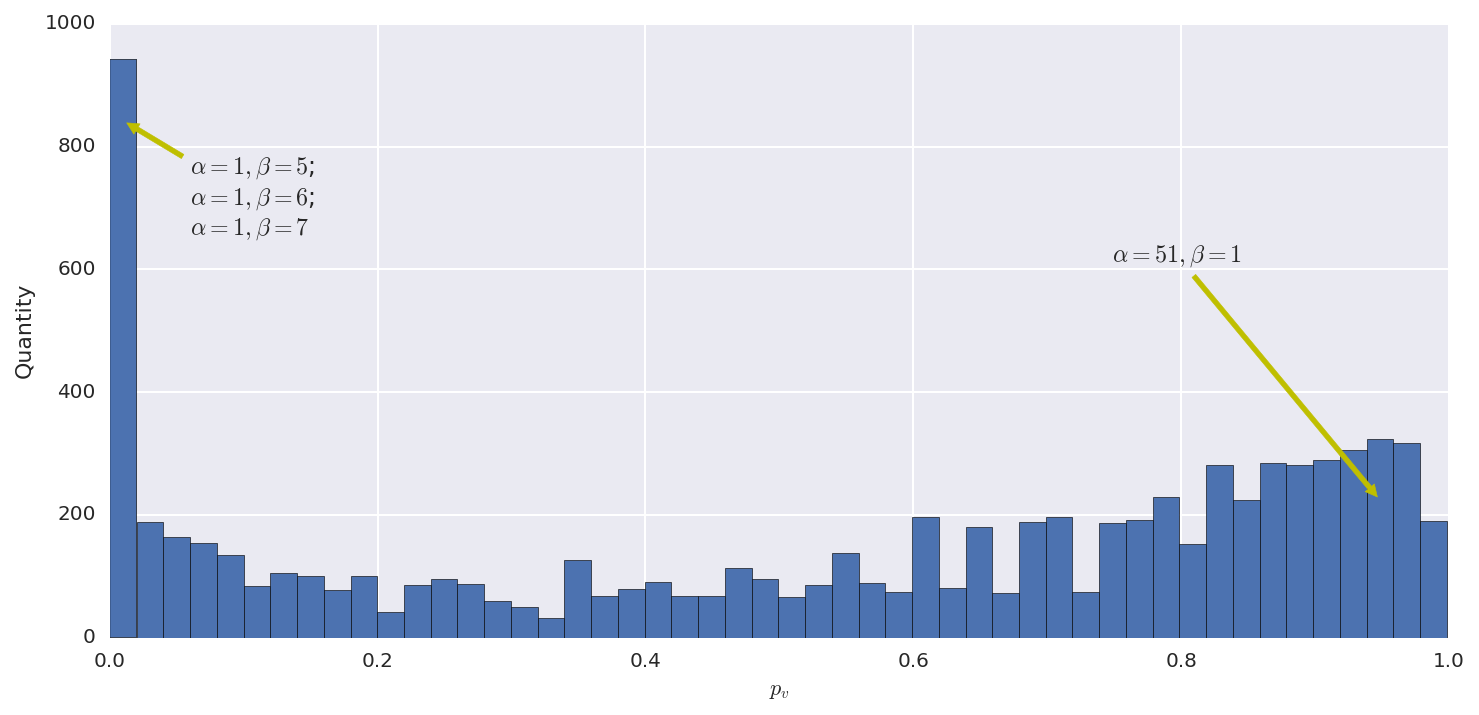
\includegraphics[width=\textwidth]{figures/bayes/3contacts/hist_calls.png}
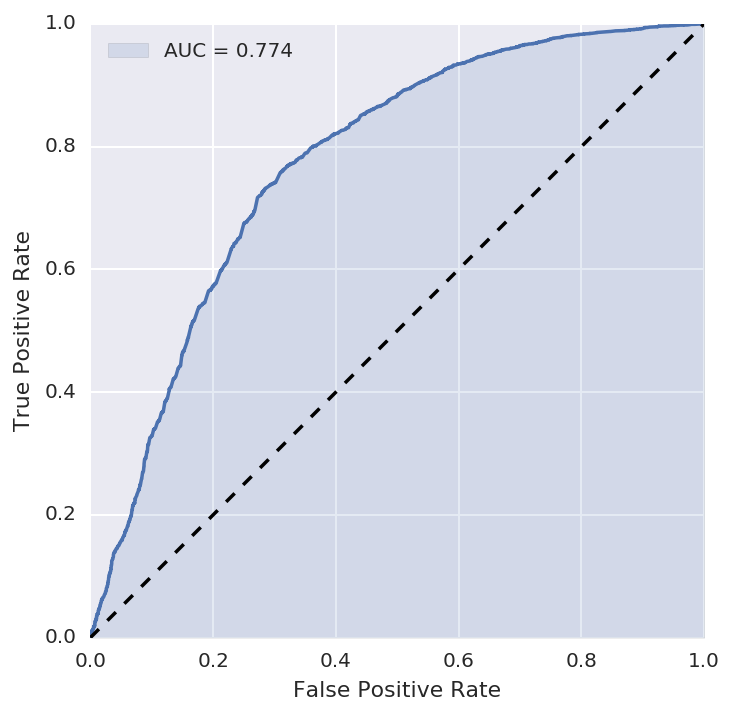
\includegraphics[width=.49\textwidth]{figures/bayes/3contacts/roc_calls.png}
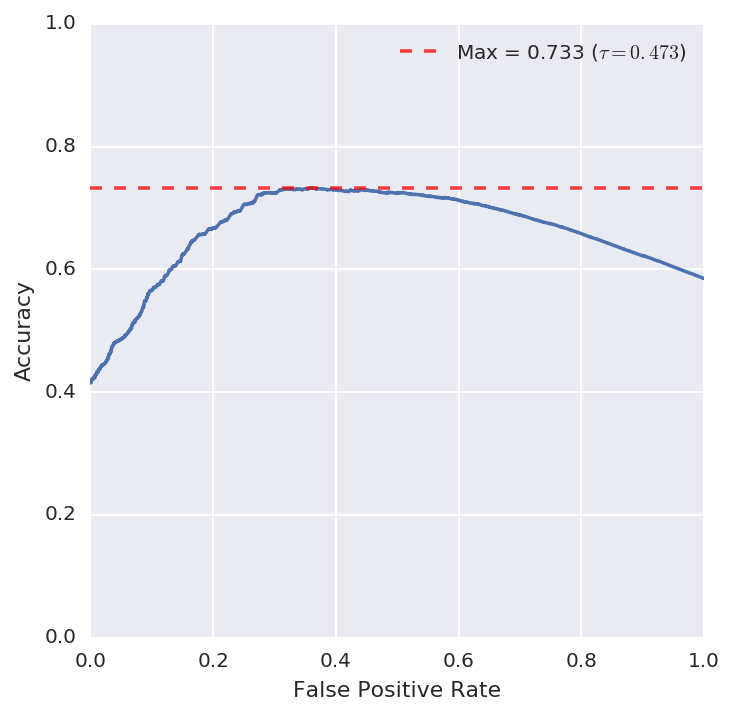
\includegraphics[width=.49\textwidth]{figures/bayes/3contacts/accuracy_calls.png}
\end{center}

Using $I^{\calls} \subseteq \Upsilon^{\calls}$ and $\varpi = \calls$ results in a predictor where both the \emph{Area Under the Curve} and the \emph{Accuracy} are higher than in all predictors that use every possible user. However, this data predicts less users and is strictly worse than the one predicting by Contacts presented in the following section.

\subsubsection{Inferring by Degree on Users with at least 3 Contacts}

\begin{center}
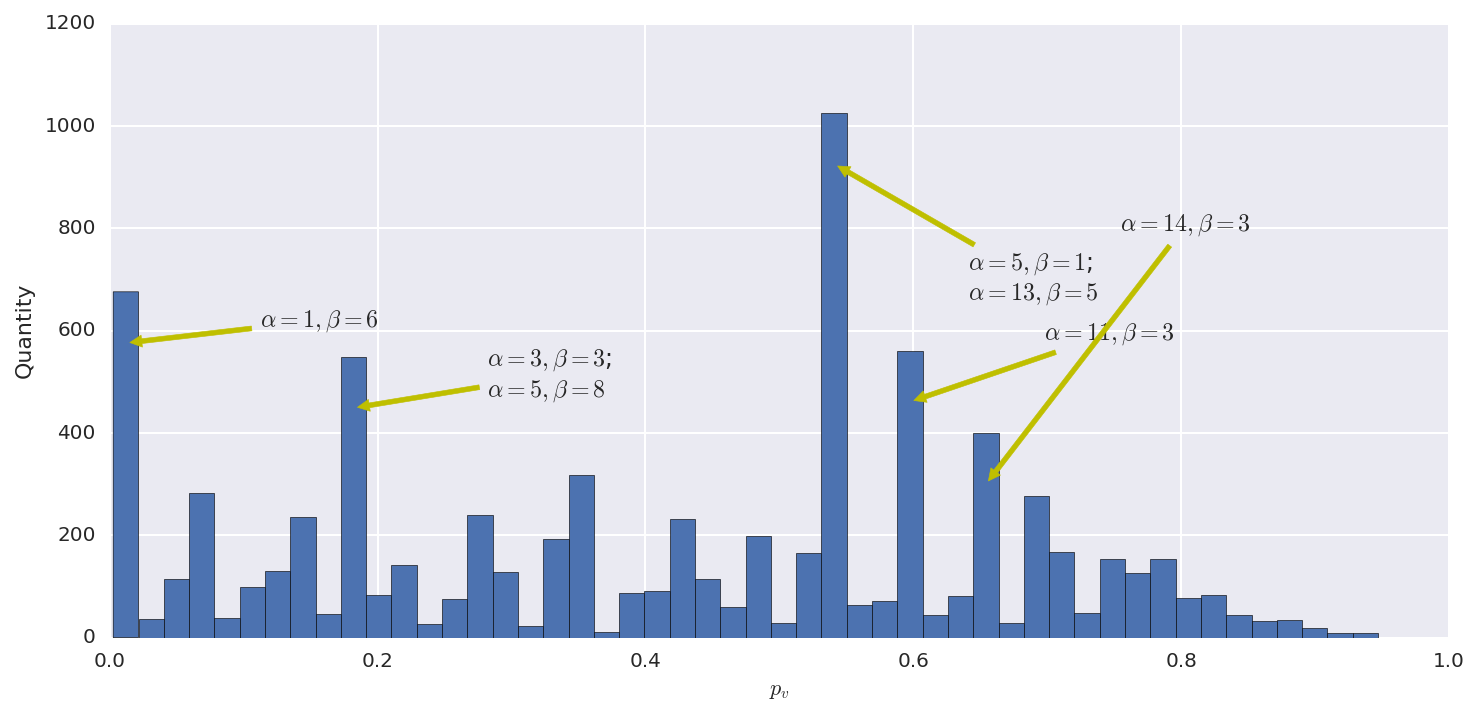
\includegraphics[width=\textwidth]{figures/bayes/3contacts/hist_contacts.png}
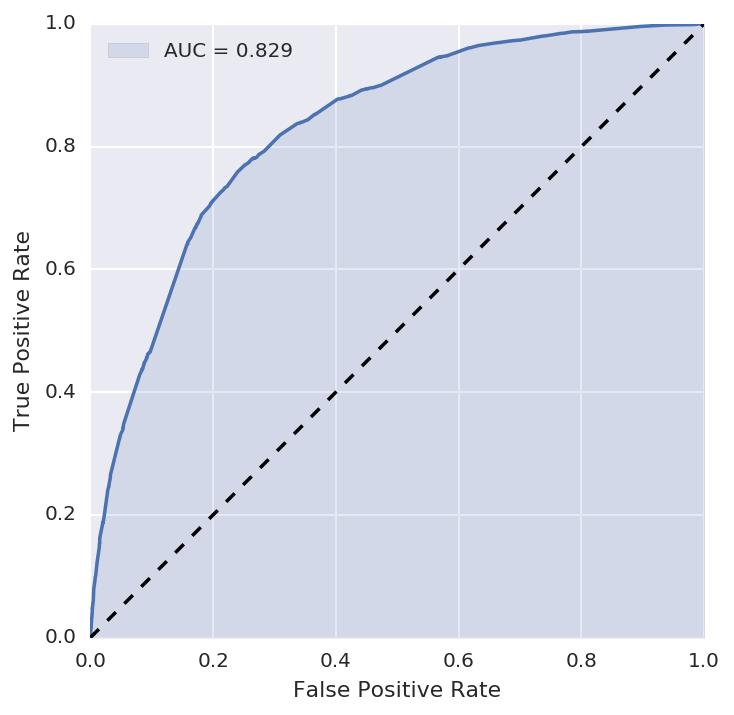
\includegraphics[width=.49\textwidth]{figures/bayes/3contacts/roc_contacts.png}
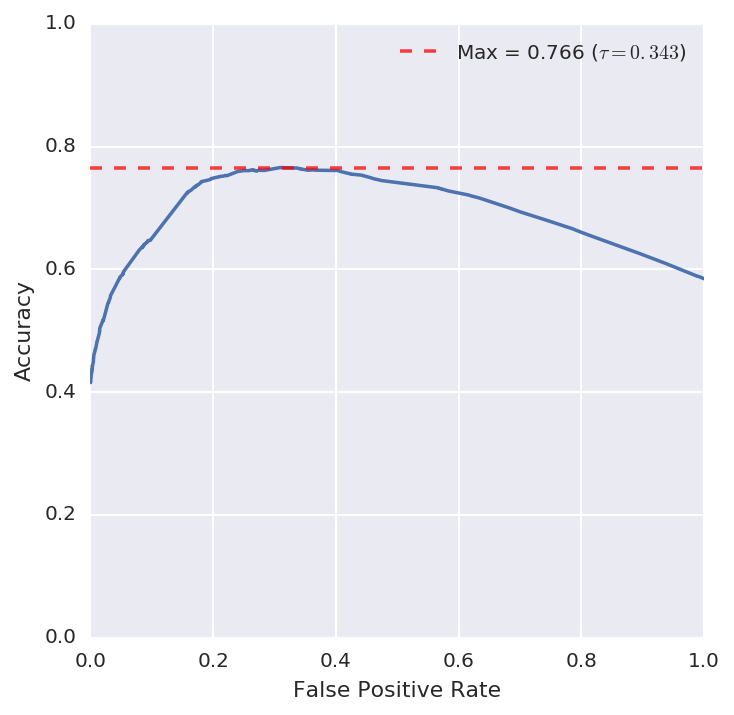
\includegraphics[width=.49\textwidth]{figures/bayes/3contacts/accuracy_contacts.png}
\end{center}

This dataset results in the best possible predictor for a reasonable subset of the users. Both the \emph{Area Under the Curve} and the \emph{Accuracy} are higher than for all other predictors: $\AUC = 0.829$, $\Accuracy = 0.766$, $\FPR = 123$, $\TPR = 123$, $\Precision = 123$, $\Recall = 123$, $F_1 = 123$, and $F_4 = 123$.

All of those values are considerably better than any other predictor in this page at the cost of using only a small subset of the possible users. This is interesing as it's exactly the same subset as the one used in~\cite{fixmanasonam2016}, and it scores significantly higher in all the metrics.
